\chapter{Budowa dwukołowego robota balansującego i implementacja algorytmów}
\label{chap:budowa}

\begin{figure}[h!]
    \centering
    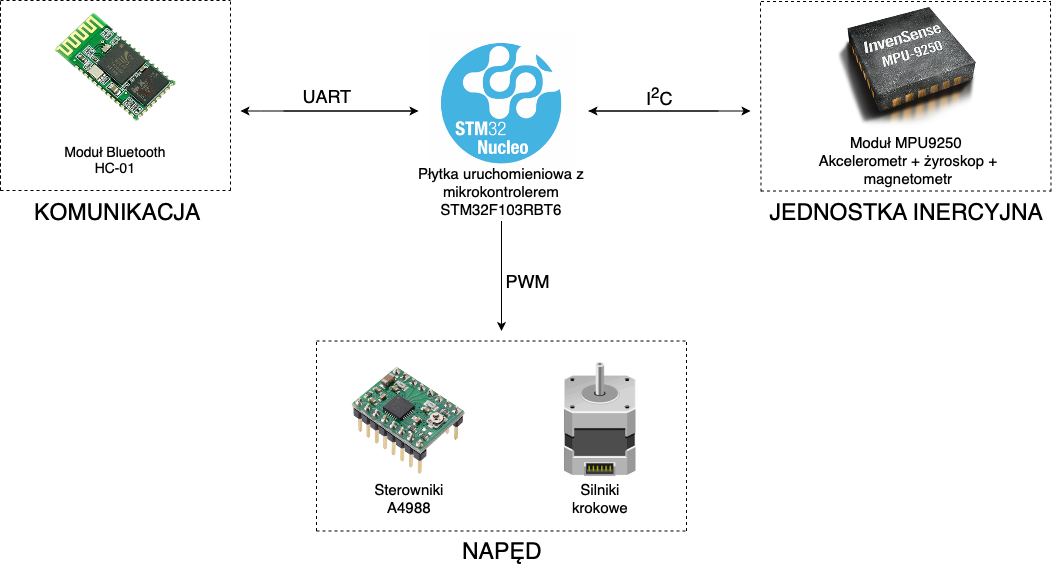
\includegraphics[width=1\textwidth]{Rysunki/Rozdzial05/Platforma_sprzetowa.png}
    \caption{Wykorzystane w budowie moduły}
    \label{Moduly}
\end{figure}

%----------------------------------------------------------------------------------------------------------------
\section{Konstrukcja mechaniczna}

%----------------------------------------------------------------------------------------------------------------
\section{Układ elektroniczny}

\subsection{Zasilanie}
...

\subsection{Jednostka inercyjna MPU9250}
...

\subsection{Moduł Bluetooth HC--05}
...

\subsection{Silniki krokowe oraz sterowniki A4988}
...

%----------------------------------------------------------------------------------------------------------------
\section{Konfiguracja mikrokontrolera i peryferiów}

\begin{figure}[h!]
    \centering
    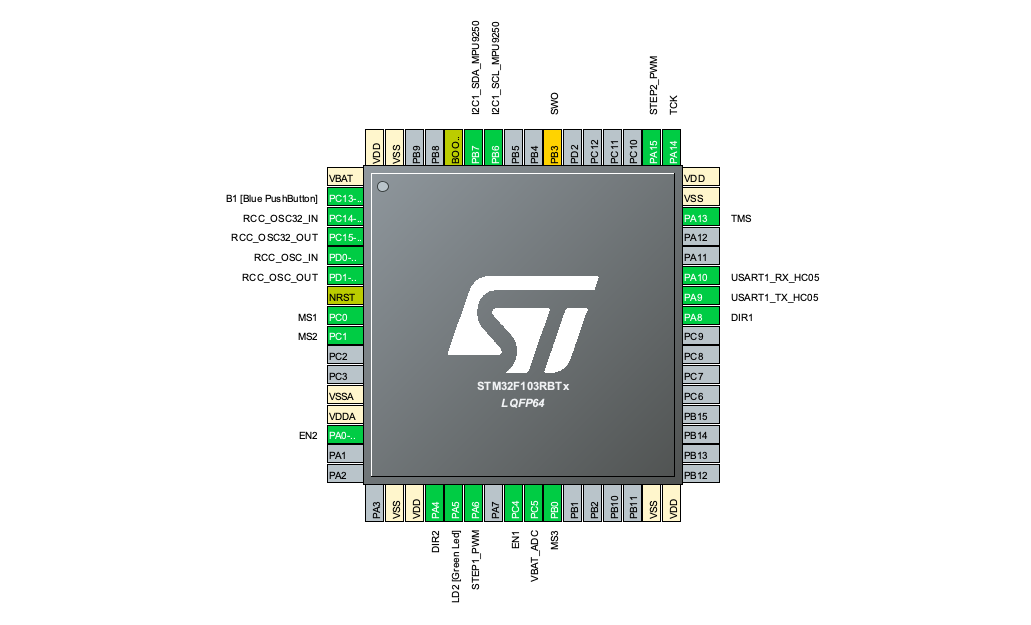
\includegraphics[width=0.5\textwidth]{Rysunki/Rozdzial05/Pinout.png}
    \caption{Konfiguracja pinów mikrokontrolera}
    \label{Piny}
\end{figure}

\subsection{ADC}
...

\subsection{PWM}
...

\subsection{$\mathbf{I^{2}C}$}
...

\subsection{USART}
...

\subsection{System czasu rzeczywistego FreeRTOS}
...

%----------------------------------------------------------------------------------------------------------------
\section{Oprogramowanie}

\subsection{Struktura programu i algorytm sterowania}

\begin{figure}[h!]
    \centering
    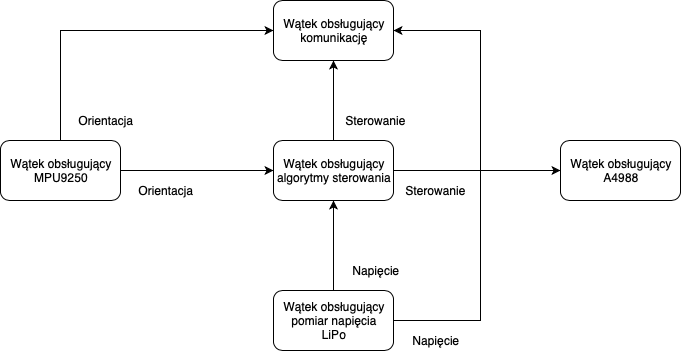
\includegraphics[width=0.5\textwidth]{Rysunki/Rozdzial05/Software.png}
    \caption{Struktura podziału programu na wątki}
    \label{Watki}
\end{figure}

\subsection{Implementacja akwizycji danych z czujników ruchu}
...

\subsection{Implementacja fuzji sygnałów}
...

\subsection{Pojedynczy regulator PID}
...

\subsection{Kaskada regulatorów PID}
...

\subsection{Obsługa silników krokowych}
...

\subsection{Pomiar stanu akumulatora}
...

\subsection{Komunikacja bezprzewodowa z komputerem}
...

\section{Testy eksperymentalne}
...